Das Testframework soll für die automatisierten Systemtests der Software der Ladesäule (sowohl mit als auch ohne Hardware) benutzt werden.

Die Anforderungen an das Testframework sind:
\begin{itemize}
    \item Der OCPP Server soll den Port selber auswählen können, um mehrere Tests parallel starten zu können.
    \item Das Verhalten von dem Testserver soll geändert werden können (auch während der Tests)
    \item Das Defaultverhalten von dem Testserver soll parametrierbar sein (z.b. einen Benutzer hinzufügen)
    \item Alle Events, die den Zustand der getesteten Ladesäule aufdecken, sollen beobachtbar sein (z.B. OCPP Nachrichten, Netzwerkevents usw.)
\end{itemize}

Die nachfolgende Abbildung \ref{fig:summaryDiagrammFramework} ist ein Übersichtdiagramm der Framework-Anwendung.
\begin{figure}[H]
    \centering
    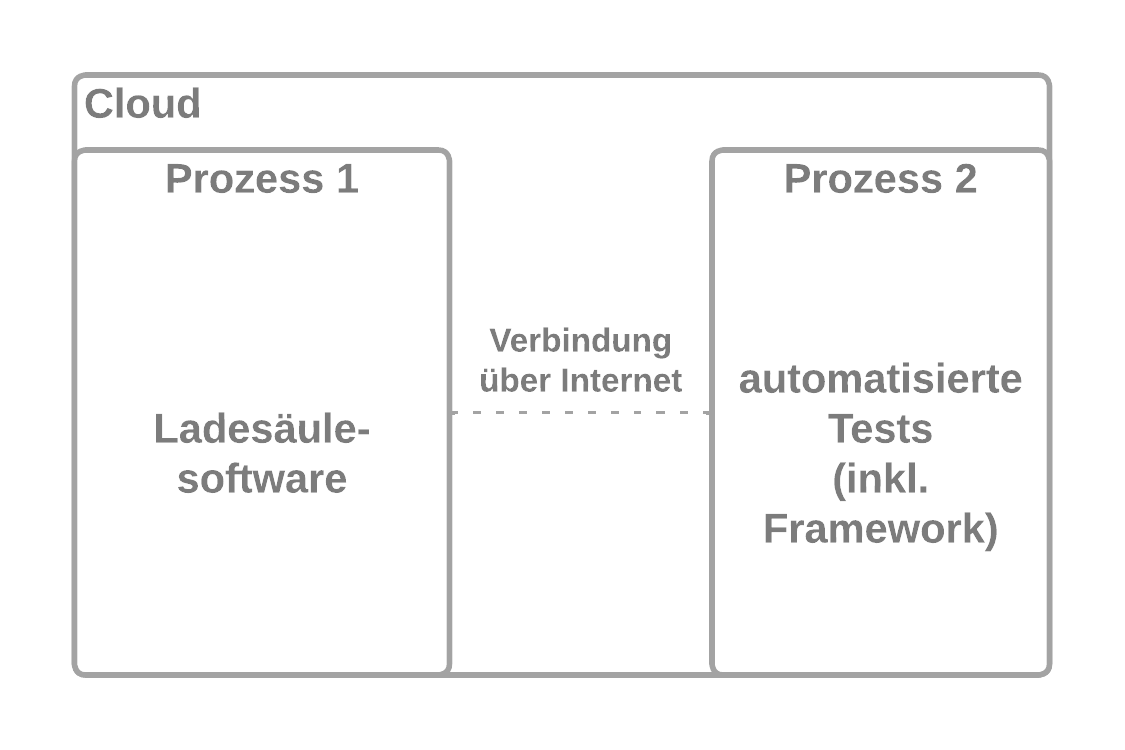
\includegraphics[width=1\textwidth]{./images/Framework.png}
    \caption[Übersichtdiagramm der Framework-Anwendung]{Übersichtdiagramm der Framework-Anwendung}
    \label{fig:summaryDiagrammFramework}
\end{figure}